% ============================================================ spin polarisation, topology rules, Ovchinnikov, Lieb
\section{Spin polarisation}

\begin{frame}{Dynamic spin polarisation}
  \begin{columns}[c]
    \column{0.55\textwidth}
    \begin{paperclaim}
      ``A damped spin wave so formed generates ferromagnetic coupling between the spins separated by an odd number
      of sites, and antiferromagnetic between those separated by an even number of sites, thus yielding the
      topology rules of spin coupling.'' (p.\ 443)
    \end{paperclaim}
    \column{0.4\textwidth}
    \centering
    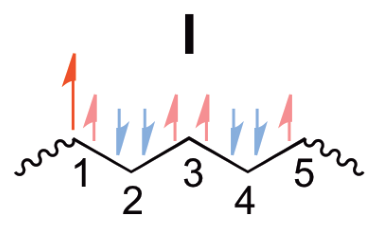
\includegraphics[width=0.72\linewidth]{scheme01_dynamic_spin_polarization.png}
    \vskip0.1cm
    {\scriptsize\cmuted{Scheme 1}}
  \end{columns}
  \onslide<2->{
  \begin{enumerate}
    \item Hückel: the unpaired electron sits in the NBMO, which is \cgold{zero on unstarred atoms}
    \item<3-> add on-site repulsion $U$: an $\uparrow$ electron pushes $\downarrow$ density onto its neighbours
    \item<4-> negative spin density appears between positive ones: \cgold{a correlation effect}
  \end{enumerate}}
  \symbolstrip{spin density $\rho_s=\rho_\uparrow-\rho_\downarrow$ on each atom \quad ferromagnetic: parallel spins; antiferromagnetic: antiparallel \quad
    ``sites'' $=$ atoms; ``separated by an odd number of sites'' $=$ odd number of atoms in between}
\end{frame}

\begin{frame}{Measured on the pentadienyl radical}{T9: exact Hubbard diagonalisation, 5 sites, 5 electrons, $S_z=\tfrac12$}
  \begin{columns}[c]
    \column{0.6\textwidth}
    \begin{tikzpicture}
      \begin{axis}[noirplot,ybar,bar shift=0pt,width=7.4cm,height=5.0cm,bar width=13pt,ymin=-0.3,ymax=0.6,
          xtick={1,2,3,4,5},xlabel={site},ylabel={spin density $\rho_s$},ymajorgrids,xmin=0.4,xmax=5.6]
        \only<1| handout:0>{\addplot[fill=noirmuted,draw=none] coordinates {(1,0.3333) (2,-0.0000) (3,0.3333) (4,-0.0000) (5,0.3333)};}
        \only<2| handout:0>{\addplot[fill=noircyan,draw=none] coordinates {(1,0.3816) (2,-0.0682) (3,0.3730) (4,-0.0682) (5,0.3816)};}
        \only<3| handout:0>{\addplot[fill=noirgold,draw=none] coordinates {(1,0.4512) (2,-0.1823) (3,0.4621) (4,-0.1823) (5,0.4512)};}
        \only<4->{\addplot[fill=noirrose,draw=none] coordinates {(1,0.4898) (2,-0.2533) (3,0.5269) (4,-0.2533) (5,0.4898)};}
      \end{axis}
    \end{tikzpicture}
    \column{0.36\textwidth}
    \only<1| handout:0>{\cmuted{$U=0$ (Hückel):}\\ unstarred sites exactly $0$}
    \only<2| handout:0>{\ccyan{$U=t$}: small negative dips}
    \only<3| handout:0>{\cgold{$U=3t$}: $-0.18$ on sites 2, 4}
    \only<4->{\crose{$U=6t$}: $-0.25$; the ``damped spin wave''}
    \vskip0.3cm
    \onslide<4->{\small total is always $1$; positive on starred, negative on unstarred atoms}
  \end{columns}
  \symbolstrip{pentadienyl: chain of 5 carbons, one unpaired electron \quad $U/t$: strength of on-site repulsion relative to hopping \quad
    $S_z=\tfrac12$: three $\uparrow$, two $\downarrow$ electrons \quad starred sites 1, 3, 5}
\end{frame}

\begin{frame}{From bonds to topology}
  \begin{columns}[c]
    \column{0.52\textwidth}
    \begin{enumerate}
      \item strong $U$: each bond carries $J_{\text{AF}}=4t^2/U$ (kinetic exchange, Part IX)
      \item<2-> bipartite graph: every bond joins $\mathcal A$ to $\mathcal B$
      \item<3-> lowest energy: $\mathcal A$ spins one way, $\mathcal B$ spins the other (Néel)
      \item<4-> same set $\Leftrightarrow$ even number of bonds $\Leftrightarrow$ odd number of atoms in between
    \end{enumerate}
    \onslide<5->{\cgold{same set: parallel; different sets: antiparallel}}
    \column{0.45\textwidth}
    \centering
    \begin{tikzpicture}[scale=0.8]
      \foreach \k in {0,...,5} \coordinate (r\k) at ({90-60*\k}:1);
      \draw[noirmuted,line width=1pt] (r0) -- (r1) -- (r2) -- (r3) -- (r4) -- (r5) -- cycle;
      \draw[noirmuted,line width=1pt] (r0) -- (90:1.9) (r2) -- (-30:1.9);
      \fill[noirrose] (90:1.9) circle (0.12); \fill[noirrose] (-30:1.9) circle (0.12);
      \node[font=\scriptsize,text=noirrose] at (0,-2.3) {meta: 3 atoms between};
      \node[font=\scriptsize,text=noirrose] at (0,-2.85) {parallel, triplet};
      \onslide<5->{
      \begin{scope}[xshift=4.2cm]
        \foreach \k in {0,...,5} \coordinate (q\k) at ({90-60*\k}:1);
        \draw[noirmuted,line width=1pt] (q0) -- (q1) -- (q2) -- (q3) -- (q4) -- (q5) -- cycle;
        \draw[noirmuted,line width=1pt] (q0) -- (90:1.9) (q3) -- (-90:1.9);
        \fill[noirrose] (90:1.9) circle (0.12); \fill[noirblue] (-90:1.9) circle (0.12);
        \node[font=\scriptsize,text=noirblue] at (0,-2.3) {para: 4 atoms between};
        \node[font=\scriptsize,text=noirblue] at (0,-2.85) {antiparallel, singlet};
      \end{scope}}
    \end{tikzpicture}
  \end{columns}
  \symbolstrip{Néel state: neighbours antiparallel everywhere \quad meta / para: $m$- / $p$-xylylene, CH$_2$ groups at ring positions 1,3 / 1,4 \quad
    a path of an even number of bonds returns to the same set}
\end{frame}

\begin{frame}{Ovchinnikov's rule, and Lieb's theorem behind it}
  \begin{columns}[c]
    \column{0.5\textwidth}
    count the Néel arrangement: $n_A$ up, $n_B$ down
    {\[
      S=\tfrac12\,|n_A-n_B|
    \]}
    \onslide<2->{\small Ovchinnikov's rule, as the review states it (p.\ 443): the most spin-alternant determinant ``is expected to have the lowest
      energy and the highest contribution''}
    \onslide<3->{
    \begin{keyresult}[Lieb, Phys.\ Rev.\ Lett.\ 62, 1201 (1989)]
      repulsive Hubbard model, bipartite graph, half filling, any $U>0$: unique ground state with
      $S=\tfrac12\bigl||\mathcal B|-|\mathcal A|\bigr|$
    \end{keyresult}}
    \column{0.46\textwidth}
    \onslide<4->{
    \small
    \begin{tabular}{lccc}
      \toprule
      T9 ($U=3t$) & $n_A/n_B$ & rule & exact\\
      \midrule
      CBD & 2/2 & 0 & \cgreen{0}\\
      TMM & 1/3 & 1 & \cgreen{1}\\
      TME & 3/3 & 0 & \cgreen{0}\\
      MX & 3/5 & 1 & \cgreen{1}\\
      TriMB & 3/6 & $\tfrac32$ & \cgreen{$\tfrac32$}\\
      TetraMB & 5/5 & 0 & \cgreen{0}\\
      $p$-xylylene & 4/4 & 0 & \cgreen{0}\\
      \bottomrule
    \end{tabular}}
    \onslide<5->{\scriptsize\crose{TriMB: the review (p.\ 444) groups it with MX as having ``triplet ground states''; three unpaired
      electrons give a \emph{quartet} ($S=\tfrac32$).}}
  \end{columns}
  \symbolstrip{$n_A,n_B$: starred / unstarred atom counts \quad half filling: one $\pi$ electron per carbon \quad
    $S=0$ singlet, $1$ triplet, $\tfrac32$ quartet \quad rule $=$ Ovchinnikov count; exact $=$ our diagonalisation}
\end{frame}

\begin{frame}{Disjoint diradicals: who picks the singlet?}
  \begin{columns}[c]
    \column{0.5\textwidth}
    \begin{paperclaim}
      ``In the singlet state of D$_{4h}$ CBD, the bonding $\pi$-electrons can partially localize on the same pair of
      atoms as the same-spin unpaired electrons; however, in the triplet state such advantageous spin polarization
      is not possible.'' (p.\ 443)
    \end{paperclaim}
    \column{0.46\textwidth}
    \begin{itemize}
      \item<2-> first order: $2K_{ab}=0$ (disjoint)
      \item<3-> second order: spin polarisation of the paired electrons, $\propto U^2$
      \item<4-> our scaling test: gap $\propto U^{1.97}$ (CBD), $U^{1.95}$ (TME), singlet lower
    \end{itemize}
    \onslide<5->{\okpill\ \small consistent with the spin-polarisation mechanism of the review's ref.\ 9 (Kollmar \& Staemmler,
      ``Violation of Hund's rule by spin polarization''; not accessed)}
  \end{columns}
  \symbolstrip{D$_{4h}$: square geometry \quad first order: energy from the exchange integral alone \quad
    second order: energy from mixing in excited (spin-polarised) configurations, scaling as $U^2$}
\end{frame}

\begin{frame}{Topology in the paper: Figure 4}
  \begin{columns}[c]
    \column{0.55\textwidth}
    \centering
    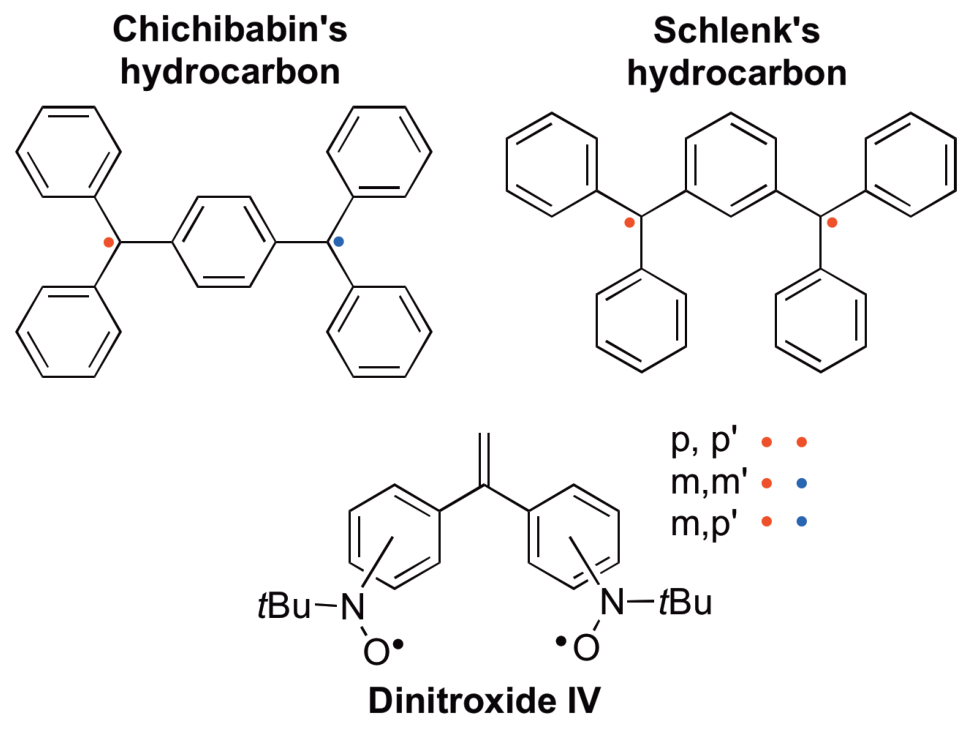
\includegraphics[width=\linewidth]{fig04_topology_driven_multiplicity.png}
    \column{0.42\textwidth}
    \begin{paperclaim}
      simple polyradicals ``can also be thought of as coupling units that sustain certain spin alignment depending on
      topology, as seen in Schlenk's and Chichibabin's hydrocarbons, or in isomers of dinitroxide IV'' (p.\ 444)
    \end{paperclaim}
    \onslide<2->{\small in Fig.\ 4, IV with $p,p'$ links: parallel spins; $m,m'$ and $m,p'$: antiparallel. Same atoms, different topology.}
  \end{columns}
  \symbolstrip{dots: \textcolor{noirrose}{rose} spin up, \textcolor{noirblue}{blue} spin down \quad $p$, $m$: para / meta attachment on each ring \quad
    Schlenk, Chichibabin: classic hydrocarbon diradicals}
\end{frame}

\begin{frame}{Tropylidene: a singlet from spin polarisation (Figure 5)}
  \begin{columns}[c]
    \column{0.5\textwidth}
    \centering
    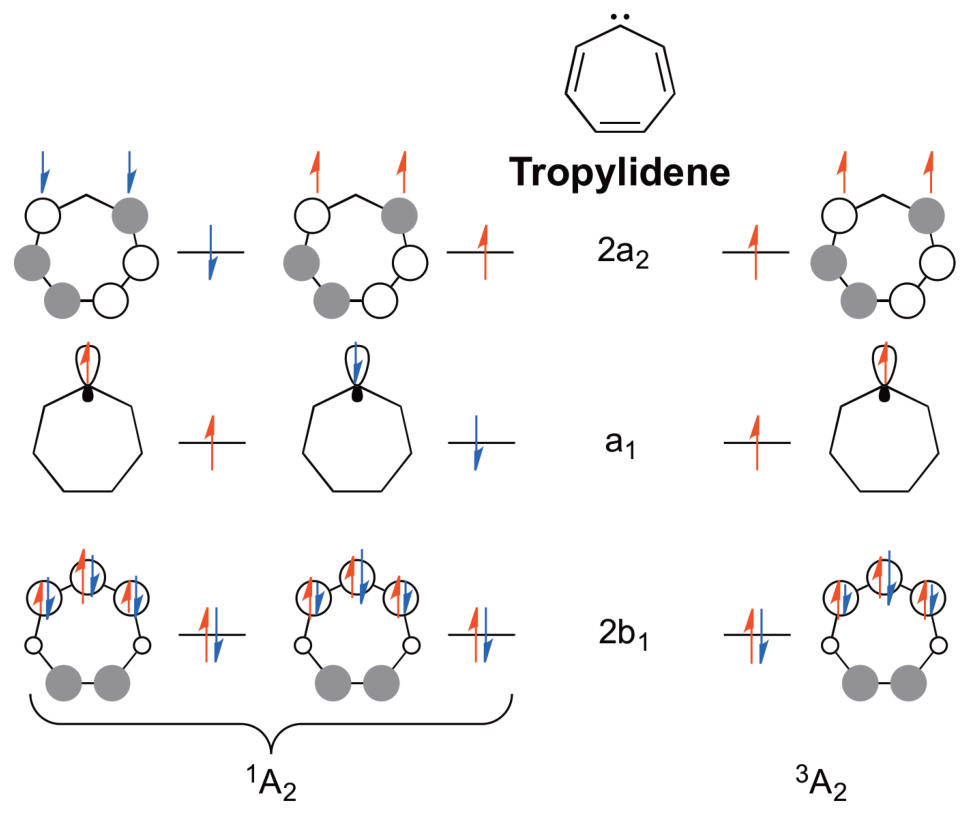
\includegraphics[width=0.92\linewidth]{fig05_tropylidene_orbitals.png}
    \column{0.47\textwidth}
    \small
    \begin{enumerate}
      \item unpaired electron in the $2a_2$ $\pi$ orbital
      \item<2-> polarises the bonding $\pi$ electrons in $2b_1$
      \item<3-> opposite spin accumulates on the carbenic carbon
      \item<4-> it couples \emph{ferromagnetically} with the electron in the orthogonal $a_1$ orbital on the same atom
      \item<5-> net result: the $^1A_2$ singlet is lower
    \end{enumerate}
    \onslide<6->{\cgold{our summary: Hund's rule obeyed locally, violated globally.}}
  \end{columns}
  \symbolstrip{tropylidene: cycloheptatrienylidene, a carbene in a 7-ring \quad $2a_2$, $2b_1$, $a_1$: orbital symmetry labels ($a_1$ in-plane, the others $\pi$) \quad
    $^1A_2$ / $^3A_2$: singlet / triplet states}
\end{frame}

\begin{frame}{Where the rules stop}
  \begin{columns}[c]
    \column{0.5\textwidth}
    \begin{itemize}
      \item Ovchinnikov / Lieb: \emph{alternant} $\pi$ systems, Hubbard/Heisenberg-type physics
      \item<2-> pyridinium V (Fig.\ 6): ionic resonance overturns the topology prediction
      \item<3-> $\sigma$--$\pi$ diradicals (didehydrotoluenes): ortho, para triplet; \emph{meta} open-shell singlet
    \end{itemize}
    \column{0.46\textwidth}
    \onslide<4->{
    \begin{paperclaim}
      ``Crucially, all of these rules are not the direct consequences of quantum mechanics and only mimic the dynamic
      and static correlation effects with the help of simplifying assumptions, thus inevitably having limited scope.'' (p.\ 443)
    \end{paperclaim}}
    \onslide<5->{\okpill\ \small fair: the topology rule is a theorem only of the Hubbard model (Lieb); the others are model heuristics}
  \end{columns}
  \symbolstrip{alternant: no odd-membered rings, so atoms split into two sets \quad $\sigma$--$\pi$ diradical: one unpaired electron in an in-plane
    $\sigma$ orbital, one in a $\pi$ orbital \quad didehydrotoluene: toluene with two H removed}
\end{frame}
